% Options for packages loaded elsewhere
\PassOptionsToPackage{unicode}{hyperref}
\PassOptionsToPackage{hyphens}{url}
\PassOptionsToPackage{dvipsnames,svgnames*,x11names*}{xcolor}
%
\documentclass[
  12pt,
]{article}
\usepackage{amsmath,amssymb}
\usepackage{lmodern}
\usepackage{iftex}
\ifPDFTeX
  \usepackage[T1]{fontenc}
  \usepackage[utf8]{inputenc}
  \usepackage{textcomp} % provide euro and other symbols
\else % if luatex or xetex
  \usepackage{unicode-math}
  \defaultfontfeatures{Scale=MatchLowercase}
  \defaultfontfeatures[\rmfamily]{Ligatures=TeX,Scale=1}
  \setmonofont[]{DejaVuSansMono.ttf}
  \setmathfont[]{texgyredejavu-math.otf}
\fi
% Use upquote if available, for straight quotes in verbatim environments
\IfFileExists{upquote.sty}{\usepackage{upquote}}{}
\IfFileExists{microtype.sty}{% use microtype if available
  \usepackage[]{microtype}
  \UseMicrotypeSet[protrusion]{basicmath} % disable protrusion for tt fonts
}{}
\makeatletter
\@ifundefined{KOMAClassName}{% if non-KOMA class
  \IfFileExists{parskip.sty}{%
    \usepackage{parskip}
  }{% else
    \setlength{\parindent}{0pt}
    \setlength{\parskip}{6pt plus 2pt minus 1pt}}
}{% if KOMA class
  \KOMAoptions{parskip=half}}
\makeatother
\usepackage{xcolor}
\IfFileExists{xurl.sty}{\usepackage{xurl}}{} % add URL line breaks if available
\IfFileExists{bookmark.sty}{\usepackage{bookmark}}{\usepackage{hyperref}}
\hypersetup{
  colorlinks=true,
  linkcolor={Maroon},
  filecolor={Maroon},
  citecolor={Blue},
  urlcolor={Blue},
  pdfcreator={LaTeX via pandoc}}
\urlstyle{same} % disable monospaced font for URLs
\usepackage[margin=0.8in,a4paper]{geometry}
\usepackage{graphicx}
\makeatletter
\def\maxwidth{\ifdim\Gin@nat@width>\linewidth\linewidth\else\Gin@nat@width\fi}
\def\maxheight{\ifdim\Gin@nat@height>\textheight\textheight\else\Gin@nat@height\fi}
\makeatother
% Scale images if necessary, so that they will not overflow the page
% margins by default, and it is still possible to overwrite the defaults
% using explicit options in \includegraphics[width, height, ...]{}
\setkeys{Gin}{width=\maxwidth,height=\maxheight,keepaspectratio}
% Set default figure placement to htbp
\makeatletter
\def\fps@figure{htbp}
\makeatother
\setlength{\emergencystretch}{3em} % prevent overfull lines
\providecommand{\tightlist}{%
  \setlength{\itemsep}{0pt}\setlength{\parskip}{0pt}}
\setcounter{secnumdepth}{-\maxdimen} % remove section numbering
% \pagestyle{empty}
\usepackage{helvet}
\usepackage{fontspec}
\usepackage{hyperref}
\usepackage{enumitem}
\usepackage{amsfonts}


\setmainfont{Arial}
\setsansfont{Arial}

\hypersetup{
  pdftitle={Sample Report},
  pdfauthor={yash2002109},
  pdfsubject={pypandoc},
  pdfkeywords={pypandoc,pdf,xelatex}
}
% set bullets
\setlist[itemize,1]{label=$\bullet$}
\setlist[itemize,2]{label=$\circ$}
\setlist[itemize,3]{label=$\star$}

%Begin each new markdown from new page
\usepackage{sectsty}
\sectionfont{\clearpage}
\ifLuaTeX
  \usepackage{selnolig}  % disable illegal ligatures
\fi

\author{}
\date{}

\begin{document}

{
\hypersetup{linkcolor=}
\setcounter{tocdepth}{1}
\tableofcontents
}
\hypertarget{technical-fork}{%
\section{Technical Fork}\label{technical-fork}}

Question: What are a number of technical forks of an open source project
on code development platforms?

\hypertarget{description}{%
\subsection{Description}\label{description}}

A technical fork is a distributed version control copy of a project. The
number of technical forks indicates the number of copies of a project on
the same code development platform.

\hypertarget{objectives}{%
\subsection{Objectives}\label{objectives}}

The objective of the Technical Fork metric is to ascertain how many
copies of a project exist on a code development platform. Analysis of
technical forks may provide insight into forking intentions (different
types of forks such as contributing, and non-contributing forks).

\hypertarget{implementation}{%
\subsection{Implementation}\label{implementation}}

\hypertarget{filters}{%
\subsubsection{Filters}\label{filters}}

\begin{itemize}
\tightlist
\item
  Time Period (e.g., Weekly, Monthly, Annually)\\
\item
  Ratio of contributing fork to total forks (A contributing fork is a
  fork that has opened a change request against the original
  repository.)\\
\item
  Ratio of non-contributing fork to total forks (A non-contributing fork
  is a fork that has never opened a change request against the original
  repository.)
\end{itemize}

\hypertarget{visualizations}{%
\subsubsection{Visualizations}\label{visualizations}}

\textbf{Augur Implementation}\\
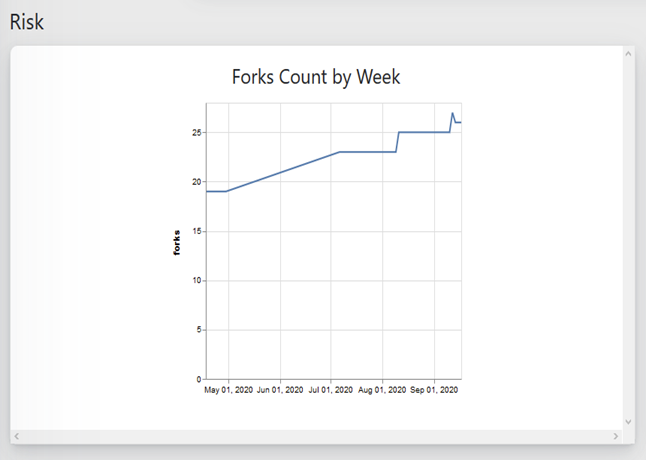
\includegraphics{images/technical-fork_augur-fork.png}

\textbf{GrimoireLab Implementation}\\
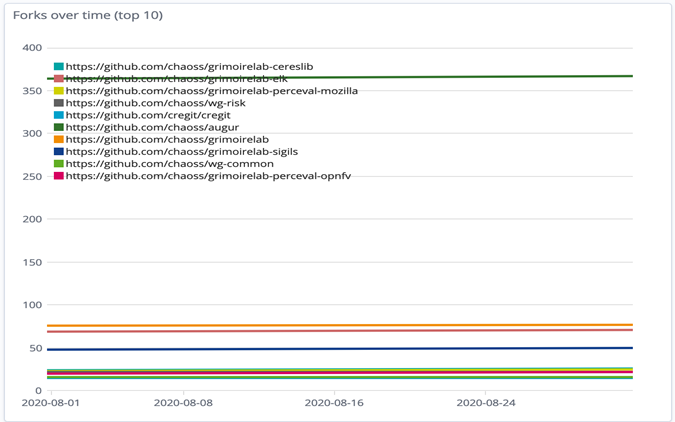
\includegraphics{images/technical-fork_grimoirelab-fork.png}

\hypertarget{tools-providing-the-metric}{%
\subsubsection{Tools Providing the
Metric}\label{tools-providing-the-metric}}

\begin{itemize}
\tightlist
\item
  Augur\\
\item
  GrimoireLab
\end{itemize}

\hypertarget{data-collection-strategies}{%
\subsubsection{Data Collection
Strategies}\label{data-collection-strategies}}

\textbf{Github API}\\
\url{https://developer.github.com/v3/repos/forks/\#list-forks}

\textbf{GitLab API}\\
\url{https://docs.gitlab.com/ee/api/projects.html\#list-forks-of-a-project}

\textbf{Bitbucket API}\\
\url{https://developer.atlassian.com/bitbucket/api/2/reference/resource/repositories/\%7Bworkspace\%7D/\%7Brepo_slug\%7D/forks}

\hypertarget{references}{%
\subsection{References}\label{references}}

\url{https://help.github.com/en/enterprise/2.13/user/articles/fork-a-repo}
\url{https://opensource.com/article/17/12/fork-clone-difference}

\hypertarget{types-of-contributions}{%
\section{Types of Contributions}\label{types-of-contributions}}

Question: What types of contributions are being made?

\hypertarget{description-1}{%
\subsection{Description}\label{description-1}}

Multiple, varied contributions make an open source project healthy. Many
projects have community members who do not write code but contribute in
equally valuable ways by managing the community, triaging bugs,
evangelizing the project, supporting users, or helping in other ways.

\hypertarget{objectives-1}{%
\subsection{Objectives}\label{objectives-1}}

A variety of contribution types can demonstrate that a project is mature
and well-rounded with sufficient activity to support all aspects of the
project, and enable paths to leadership that are supportive of a variety
of contribution types and people with varying expertise beyond coding.

\hypertarget{implementation-1}{%
\subsection{Implementation}\label{implementation-1}}

How contributions are defined, quantified, tracked and made public is a
challenging question. Answers may be unique to each project and the
following suggestions are a starting point. As a general guideline, it
is difficult to compare different contribution types with each other and
they might better be recognized independently.

\begin{itemize}
\tightlist
\item
  The following list can help with identifying contribution types:

  \begin{itemize}
  \tightlist
  \item
    Writing Code
  \item
    Reviewing Code
  \item
    Bug Triaging
  \item
    Quality Assurance and Testing
  \item
    Security-Related Activities
  \item
    Localization/L10N and Translation
  \item
    Event Organization
  \item
    Documentation Authorship
  \item
    Community Building and Management
  \item
    Teaching and Tutorial Building
  \item
    Troubleshooting and Support
  \item
    Creative Work and Design
  \item
    User Interface, User Experience, and Accessibility
  \item
    Social Media Management
  \item
    User Support and Answering Questions
  \item
    Writing Articles
  \item
    Public Relations - Interviews with Technical Press
  \item
    Speaking at Events
  \item
    Marketing and Campaign Advocacy
  \item
    Website Development
  \item
    Legal Council
  \item
    Financial Management
  \end{itemize}
\end{itemize}

\hypertarget{data-collection-strategies-1}{%
\subsubsection{Data Collection
Strategies}\label{data-collection-strategies-1}}

\begin{itemize}
\tightlist
\item
  \textbf{Interview or Survey:} Ask community members to recognize
  others for their contributions to recognize contribution types that
  have previously not been considered.

  \begin{itemize}
  \tightlist
  \item
    Who in the project would you like to recognize for their
    contributions? What did they contribute?
  \end{itemize}
\item
  \textbf{Observe project:} Identify and recognize leads of different
  parts of the project.

  \begin{itemize}
  \tightlist
  \item
    What leaders are listed on the project website or in a repository?
  \end{itemize}
\item
  \textbf{Capture Non-code Contributions:} Track contributions through a
  dedicated system, e.g., an issue tracker.

  \begin{itemize}
  \tightlist
  \item
    Logging can include custom information a project wants to know about
    non-code contributions to recognize efforts.
  \item
    Proxy contributions through communication channel activity. For
    example, If quality assurance members (QA) have their own mailing
    list, then activity around QA contributions can be measured by proxy
    from mailing list activity.
  \end{itemize}
\item
  \textbf{Collect Trace Data:} Measure contributions through
  collaboration tool log data.

  \begin{itemize}
  \tightlist
  \item
    For example, code contributions can be counted from a source code
    repository, wiki contributions can be counted from a wiki edit
    history, and email messages can be counted from an email archive
  \end{itemize}
\item
  \textbf{Automate Classification:} Train an artificial intelligence
  (AI) bot to detect and classify contributions.

  \begin{itemize}
  \tightlist
  \item
    An AI bot can assist in categorizing contributions, for example,
    help requests vs. support provided, or feature request vs. bug
    reporting, especially if these are all done in the same issue
    tracker.
  \end{itemize}
\end{itemize}

\emph{Other considerations:}

\begin{itemize}
\tightlist
\item
  Especially with automated reports, allow community members to opt-out
  and not appear on the contribution reports.
\item
  Acknowledge imperfect capture of contribution types and be explicit
  about what types of contributions are included.
\item
  As a project evolves, methods for collecting types of contributions
  will need to adapt. For example, when an internationalization library
  is exchanged, project activity around localization conceivably
  produces different metrics before and after the change.
\item
  Account for activity from bots when mining contribution types at large
  scale.
\end{itemize}

\hypertarget{references-1}{%
\subsection{References}\label{references-1}}

\begin{itemize}
\tightlist
\item
  \url{https://medium.com/@sunnydeveloper/revisiting-the-word-recognition-in-foss-and-the-dream-of-open-credentials-d15385d49447}
\item
  \url{https://24pullrequests.com/contributing}
\item
  \url{https://smartbear.com/blog/test-and-monitor/14-ways-to-contribute-to-open-source-without-being/}
\item
  \url{https://wiki.openstack.org/wiki/AUCRecognition}
\item
  \url{https://www.drupal.org/drupalorg/blog/a-guide-to-issue-credits-and-the-drupal.org-marketplace}
\end{itemize}

\hypertarget{activity-dates-and-times}{%
\section{Activity Dates and Times}\label{activity-dates-and-times}}

Question: What are the dates and timestamps of when contributor
activities occur?

\hypertarget{description-2}{%
\subsection{Description}\label{description-2}}

Individuals engage in activities in open source projects at various
times of the day. This metric is aimed at determining the dates and
times of when individual activities were completed. The data can be used
to probabilistically estimate where on earth contributions come from in
cases where the time zone is not UTC.

\hypertarget{objectives-2}{%
\subsection{Objectives}\label{objectives-2}}

\begin{itemize}
\tightlist
\item
  Improve transparency for employers about when organizational employees
  are engaging with open source projects
\item
  Improve transparency for open source project and community managers as
  to when activity is occurring
\end{itemize}

\hypertarget{implementation-2}{%
\subsection{Implementation}\label{implementation-2}}

\hypertarget{filters-1}{%
\subsubsection{Filters}\label{filters-1}}

\begin{itemize}
\tightlist
\item
  Individual by Organization
\item
  Aggregation of time by UTC time

  \begin{itemize}
  \tightlist
  \item
    Can show what times across the globe contributions are made; when
    the project is most active.
  \end{itemize}
\item
  Aggregation of time by local time

  \begin{itemize}
  \tightlist
  \item
    Can show what times of day in their local times they contribute.
    Conclusions about the If contributions are more during working
    hours, or if contributions are more during evening hours.
  \end{itemize}
\item
  Repository ID
\item
  Segment of a community, (e.g., GrimoireLab has more EU time zones
  activity and Augur more US time zones activity)
\end{itemize}

\hypertarget{visualizations-1}{%
\subsubsection{Visualizations}\label{visualizations-1}}

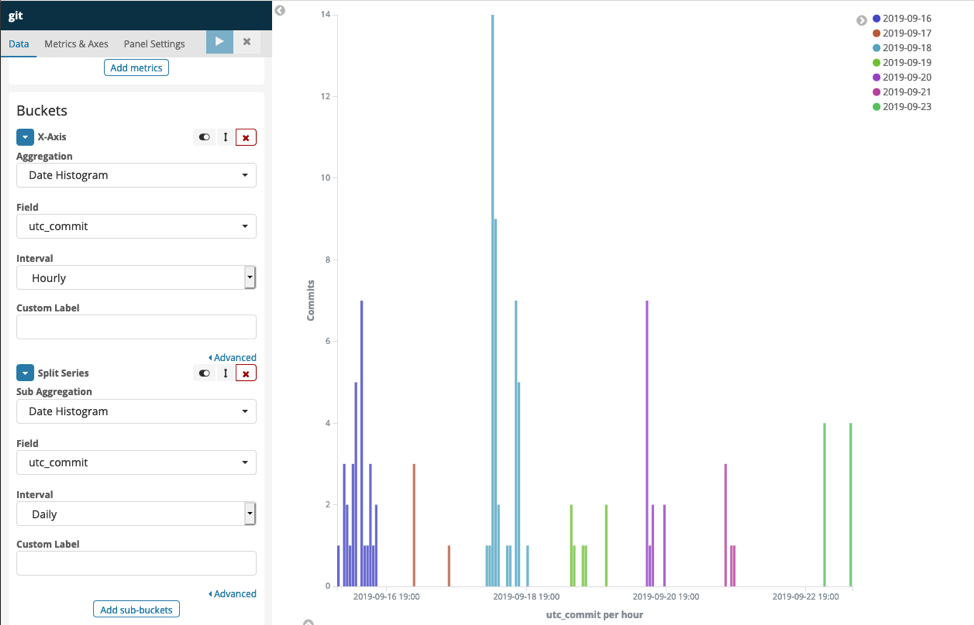
\includegraphics{images/activity-dates-and-times_1.png}
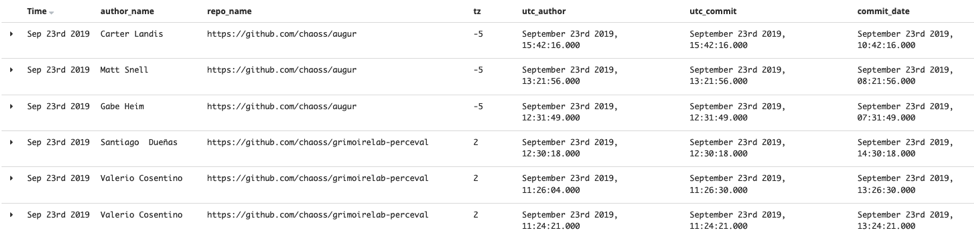
\includegraphics{images/activity-dates-and-times_2.png}
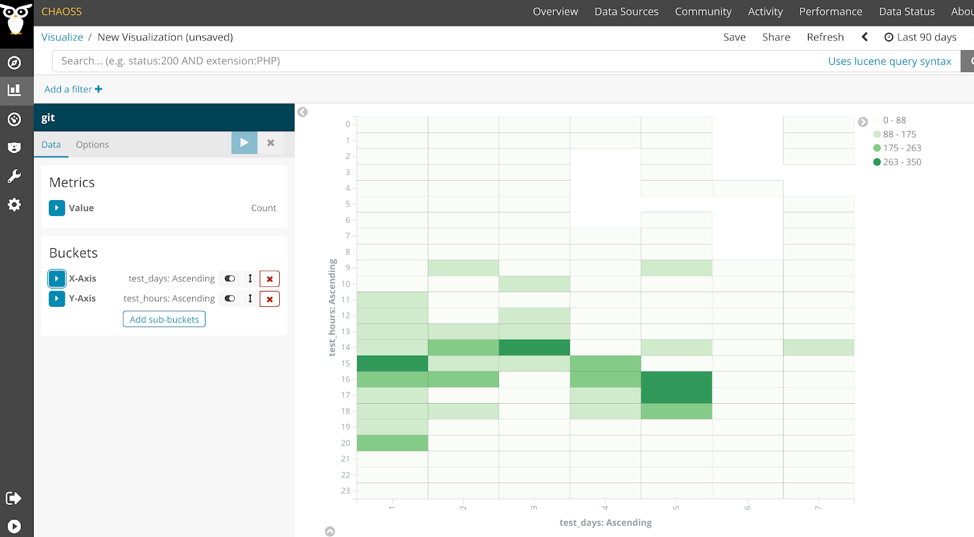
\includegraphics{images/activity-dates-and-times_3.png}
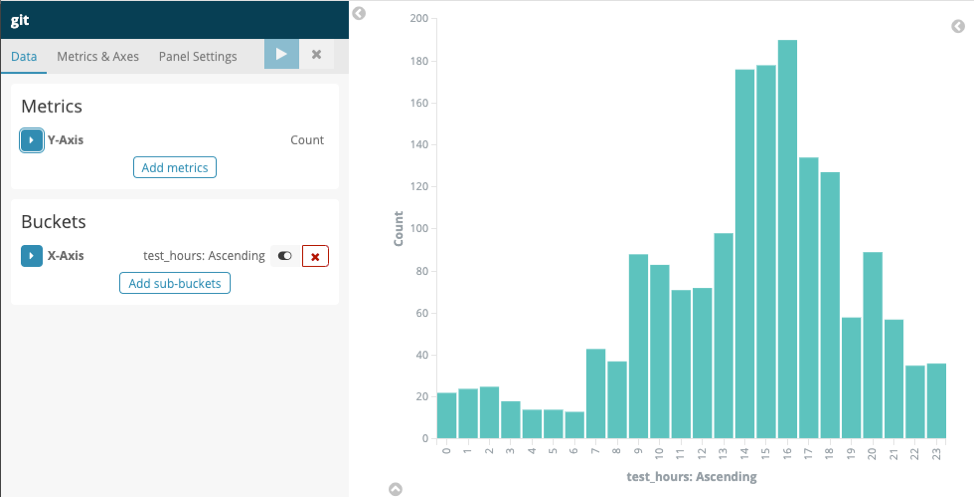
\includegraphics{images/activity-dates-and-times_4.png}

\hypertarget{tools-providing-metric}{%
\subsubsection{Tools Providing Metric}\label{tools-providing-metric}}

\href{https://chaoss.github.io/grimoirelab/}{GrimoireLab}

\href{https://docs.augur.net/\#dates-timestamps}{Augur Date/Timestamps}

\hypertarget{references-2}{%
\subsection{References}\label{references-2}}

\href{https://en.wikipedia.org/wiki/Coordinated_Universal_Time}{Coordinated
Universal Time}

\hypertarget{burstiness}{%
\section{Burstiness}\label{burstiness}}

Question: How are short timeframes of intense activity, followed by a
corresponding return to a typical pattern of activity, observed in a
project?

\hypertarget{description-3}{%
\subsection{Description}\label{description-3}}

There are a number of reasons that may prompt a sudden increase or
decrease in the amount of activity within a repository. These increases
and decreases appear both as a sudden change in activity against the
average amount of activity. Burstiness is a way of understanding the
cycle of activity in existing metrics, like issues, merge requests,
mailing lists, commits, or comments. Examples of root causes for bursts
in activity include:

\begin{itemize}
\tightlist
\item
  Release cycles
\item
  Global pandemics
\item
  Hackathon activities
\item
  Mentorship programs
\item
  Conferences, meetups, and other events where tools are presented
\item
  Conventional and social media announcements and mentions
\item
  Critical bugs as raising awareness and getting people's attention
\item
  Community design meetings or brainstorming meetings to address a
  particular issue
\item
  Community members show up from another community that is relying on
  your project (e.g., dependencies)
\end{itemize}

\hypertarget{objectives-3}{%
\subsection{Objectives}\label{objectives-3}}

\begin{itemize}
\tightlist
\item
  To identify impacts of root causes of a burst in activity
\item
  To provide awareness when project activity unknowingly goes up
\item
  To help capture the meaningfulness of increases or decreases in
  project activity
\item
  To help the community and maintainers prepare for future bursts that
  follow a pattern
\item
  To help measure the impact of influential external activities
\item
  To differentiate skewed activity versus normal activity
\end{itemize}

\hypertarget{implementation-3}{%
\subsection{Implementation}\label{implementation-3}}

\hypertarget{filters-2}{%
\subsubsection{Filters}\label{filters-2}}

\begin{itemize}
\tightlist
\item
  Stars
\item
  Forks
\item
  Issues or bug reports
\item
  Labels
\item
  Downloads
\item
  Release Tags
\item
  Change Requests
\item
  Mail List Traffic
\item
  Documentation additions or revisions
\item
  New Repositories
\item
  Feature Requests
\item
  Messaging Conversations
\item
  Conventional and Social Media Activity
\item
  Conference Attendance and Submissions
\end{itemize}

\hypertarget{visualizations-2}{%
\subsubsection{Visualizations}\label{visualizations-2}}

Augur:

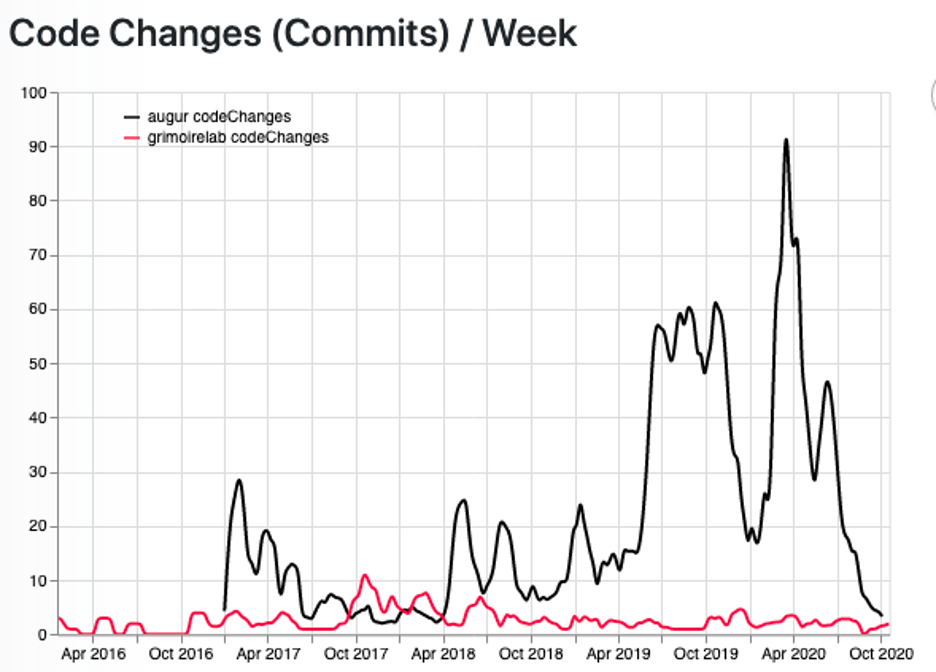
\includegraphics{images/burstiness_augur.png}

GrimoireLab:

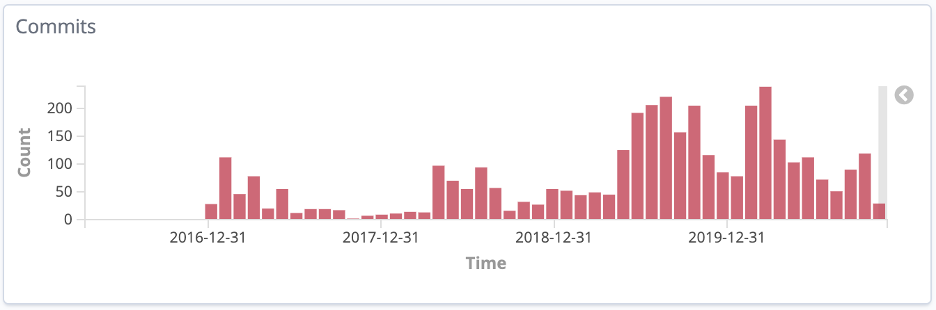
\includegraphics{images/burstiness_gl.png}

\hypertarget{tools-providing-the-metric-1}{%
\subsubsection{Tools Providing the
Metric}\label{tools-providing-the-metric-1}}

\begin{itemize}
\tightlist
\item
  Grimoire Lab
\item
  Augur
\end{itemize}

\hypertarget{data-collection-strategies-2}{%
\subsubsection{Data Collection
Strategies}\label{data-collection-strategies-2}}

\begin{itemize}
\tightlist
\item
  Quantitative

  \begin{itemize}
  \tightlist
  \item
    Time box activities identifying deviations away from some norm
  \item
    Outliers for certain thresholds, using statistics like Bollinger
    Bands to measure stability or volatility:
    \url{https://en.wikipedia.org/wiki/Bollinger_Bands}
  \end{itemize}
\item
  Qualitative Interview Questions

  \begin{itemize}
  \tightlist
  \item
    Why do you contribute more during a period of time?
  \item
    What do you believe to be the root cause for particular bursts?
  \item
    What impact do different events (e.g., hackathons, mentorship
    program, or conferences) have on project activity?
  \end{itemize}
\end{itemize}

\hypertarget{references-3}{%
\subsection{References}\label{references-3}}

This metric was inspired by the work of Goh and Barabasi (2008):
\url{https://arxiv.org/pdf/physics/0610233.pdf}

\hypertarget{review-cycle-duration-within-a-change-request}{%
\section{Review Cycle Duration within a Change
Request}\label{review-cycle-duration-within-a-change-request}}

Question: What is the duration of a review cycle within a single change
request?

\hypertarget{description-4}{%
\subsection{Description}\label{description-4}}

A change request is based on one or more review cycles. Within a review
cycle, one or more reviewers can provide feedback on a proposed
contribution. The duration of a review cycle, or the time between each
new iteration of the contribution, is the basis of this metric.

\hypertarget{objectives-4}{%
\subsection{Objectives}\label{objectives-4}}

This metric provides maintainers with insight on: Code review process
decay, as there are more iterations and review cycle durations increase.
Process bottlenecks resulting in long code review iterations. Abandoned
or semi-abandoned processes in the review cycles, where either the
maintainer or the submitter is slow in responding. Characteristics of
reviews that have different cyclic pattern lengths.

\hypertarget{implementation-4}{%
\subsection{Implementation}\label{implementation-4}}

Review Cycle Duration is measured as the time length of one review cycle
within a single change request. The duration can be calculated between:
The moment when each review cycle begins, defined as the point in time
when a change request is submitted or updated. The moment when each
review cycle ends, either because the change request was updated and
needs a new review or because it was accepted or rejected.

\hypertarget{filter}{%
\subsubsection{Filter}\label{filter}}

Average or Median Duration, optionally filtered or grouped by: Number of
people involved in review Number of comments in review Edits made to a
change request Project or program Organization making the change request
Time the change request was submitted Developers who contributed to a
change request Change request Number of review cycle on a change request
(e.g., filter by first, second, \ldots{} round)

\hypertarget{visualizations-3}{%
\subsubsection{Visualizations}\label{visualizations-3}}

\hypertarget{tools-providing-the-metric-2}{%
\subsubsection{Tools Providing the
Metric}\label{tools-providing-the-metric-2}}

\hypertarget{references-4}{%
\subsection{References}\label{references-4}}

Example of data that could be used to develop the metric:
\url{https://gerrit.wikimedia.org/r/c/mediawiki/core/+/194071}

\hypertarget{time-to-close}{%
\section{Time to Close}\label{time-to-close}}

Question: How much time passes between creating and closing an operation
such as an issue, change request, or support ticket?

\hypertarget{description-5}{%
\subsection{Description}\label{description-5}}

The time to close is the total amount of time that passes between the
creation and closing of an operation such as an issue, change request,
or support ticket. The operation needs to have an open and closed state,
as is often the case in code review processes, question and answer
forums, and ticketing systems.

Related metric:
\href{https://chaoss.community/metric-issue-resolution-duration/}{Issue
Resolution Duration}

\hypertarget{objectives-5}{%
\subsection{Objectives}\label{objectives-5}}

\begin{enumerate}
\tightlist
\item
  Determining how responsive a community is can help efforts to be
  inclusive, attract, and retain new and existing contributors.\\
\item
  Identifying characteristics of operations that impact an operation
  closing quickly or slowly (e.g., finding best practices, areas of
  improvement, assess efficiency).\\
\item
  Identifying bias for timely responses to different community
  members.\\
\item
  Detecting a change in community activity (e.g., to indicate potential
  maintainer burnout, reduction in the diversity of contributions)\\
\item
  Understand how the time to close an issue or change request is related
  to merge success or failure.
\end{enumerate}

\hypertarget{implementation-5}{%
\subsection{Implementation}\label{implementation-5}}

\hypertarget{filters-3}{%
\subsubsection{Filters}\label{filters-3}}

\begin{itemize}
\tightlist
\item
  Creator of operation (e.g., new contributor vs. maintainer)\\
\item
  First closed, final closed\\
\item
  Labels (e.g., bug vs. new feature)
\item
  Change Request Merge Status (e.g. Time to Merge or Time to Close
  without Merge)
\end{itemize}

\hypertarget{visualizations-4}{%
\subsubsection{Visualizations}\label{visualizations-4}}

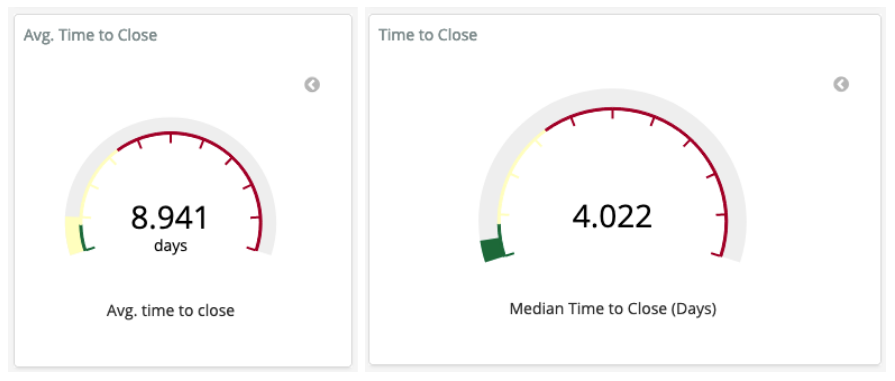
\includegraphics{images/time-to-close_1.png}

\hypertarget{tools-providing-the-metric-3}{%
\subsubsection{Tools Providing the
Metric}\label{tools-providing-the-metric-3}}

Augur implementation:

\begin{itemize}
\tightlist
\item
  \href{http://augur.osshealth.io/api_docs/\#api-Evolution-Closed_Issue_Resolution_Duration(Repo)}{Issue
  Close Duration}\\
\item
  \href{http://augur.osshealth.io/api_docs/\#api-Evolution-issue-duration-repo}{Issue
  Duration}\\
\item
  \href{http://augur.osshealth.io/api_docs/\#api-Evolution-Issue_Response_Time(Repo)}{Issue
  Response Time}
\end{itemize}

GrimoireLab implementation:

\begin{itemize}
\tightlist
\item
  \href{https://chaoss.github.io/grimoirelab-sigils/panels/github-pullrequests-efficiency/}{Pull
  Requests Efficiency}\\
\item
  \href{https://chaoss.github.io/grimoirelab-sigils/panels/github-issues-efficiency/}{Issues
  Efficiency}\\
\item
  \href{https://chaoss.github.io/grimoirelab-sigils/panels/efficiency-timing-overview/}{Efficiency:TimingOverview}
\end{itemize}

\hypertarget{data-collection-strategies-3}{%
\subsubsection{Data Collection
Strategies}\label{data-collection-strategies-3}}

The time to close metric may be contextual based on the project activity
and objectives. For example, the time to close a bug report may provide
different information than the time to close a new feature request. Data
collection strategies should address different project objectives. Other
variables that may influence these processes are:

\begin{itemize}
\tightlist
\item
  Issue Tracking Systems: the type of issue such as bug report,
  blueprint (OpenStack nomenclature), user story, feature request, epic,
  and others may influence how long this event takes to be closed. Other
  variables, such as the priority or severity may help to advance how
  quickly this event will be closed.\\
\item
  Change Request Processes: this depends on the change request
  infrastructure, as Gerrit, GitHub or mailing lists (as in the Linux
  Kernel) and may differ depending on how complicated the process is.
  For example, newcomers or advanced and experienced developers will
  proceed in different ways and with more or less time required.\\
\item
  Question and Answer Forum: this depends on the quality of the answer
  and the opinion of the person asking the question. A valid answer is
  marked, and the process is closed once the person questioning has
  successfully found a correct answer to their question.
\end{itemize}

\hypertarget{references-5}{%
\subsection{References}\label{references-5}}

\begin{itemize}
\tightlist
\item
  ``Practice P.12: Respond to all submissions'' from ``Appendix to:
  Managing Episodic Volunteers in Free/Libre/Open Source Software
  Communities'' by Ann Barcomb, Klaas-Jan Stol, Brian Fitzgerald and
  Dirk Riehle:
  \url{https://opus4.kobv.de/opus4-fau/frontdoor/index/index/docId/13519}
\end{itemize}

\hypertarget{time-to-first-response}{%
\section{Time to First Response}\label{time-to-first-response}}

Question: How much time passes between when an activity requiring
attention is created and the first response?

\hypertarget{description-6}{%
\subsection{Description}\label{description-6}}

The first response to an activity can sometimes be the most important
response. The first response shows that a community is active and
engages in conversations. A long time to respond to an activity can be a
sign that a community is not responsive. A short time to respond to an
activity can help to engage more members into further discussions and
within the community.

\hypertarget{objectives-6}{%
\subsection{Objectives}\label{objectives-6}}

Identify cadence of first response across a variety of activities,
including PRs, Issues, emails, IRC posts, etc. Time to first response is
an important consideration for new and long-time contributors to a
project along with overall project health.

\hypertarget{implementation-6}{%
\subsection{Implementation}\label{implementation-6}}

Time to first response of an activity = time first response was posted
to the activity - time the activity was created.

\hypertarget{filters-4}{%
\subsubsection{Filters}\label{filters-4}}

\begin{itemize}
\tightlist
\item
  Role of responder, e.g., only count maintainer responses
\item
  Automated responses, e.g., only count replies from real people by
  filtering bots and other automated replies
\item
  Type of Activity, e.g., issues (see metric
  \href{https://github.com/chaoss/wg-evolution/blob/master/metrics/Issue_Response_Time.md}{Issue
  Response Time}), emails, chat, change requests
\end{itemize}

\hypertarget{visualizations-5}{%
\subsubsection{Visualizations}\label{visualizations-5}}

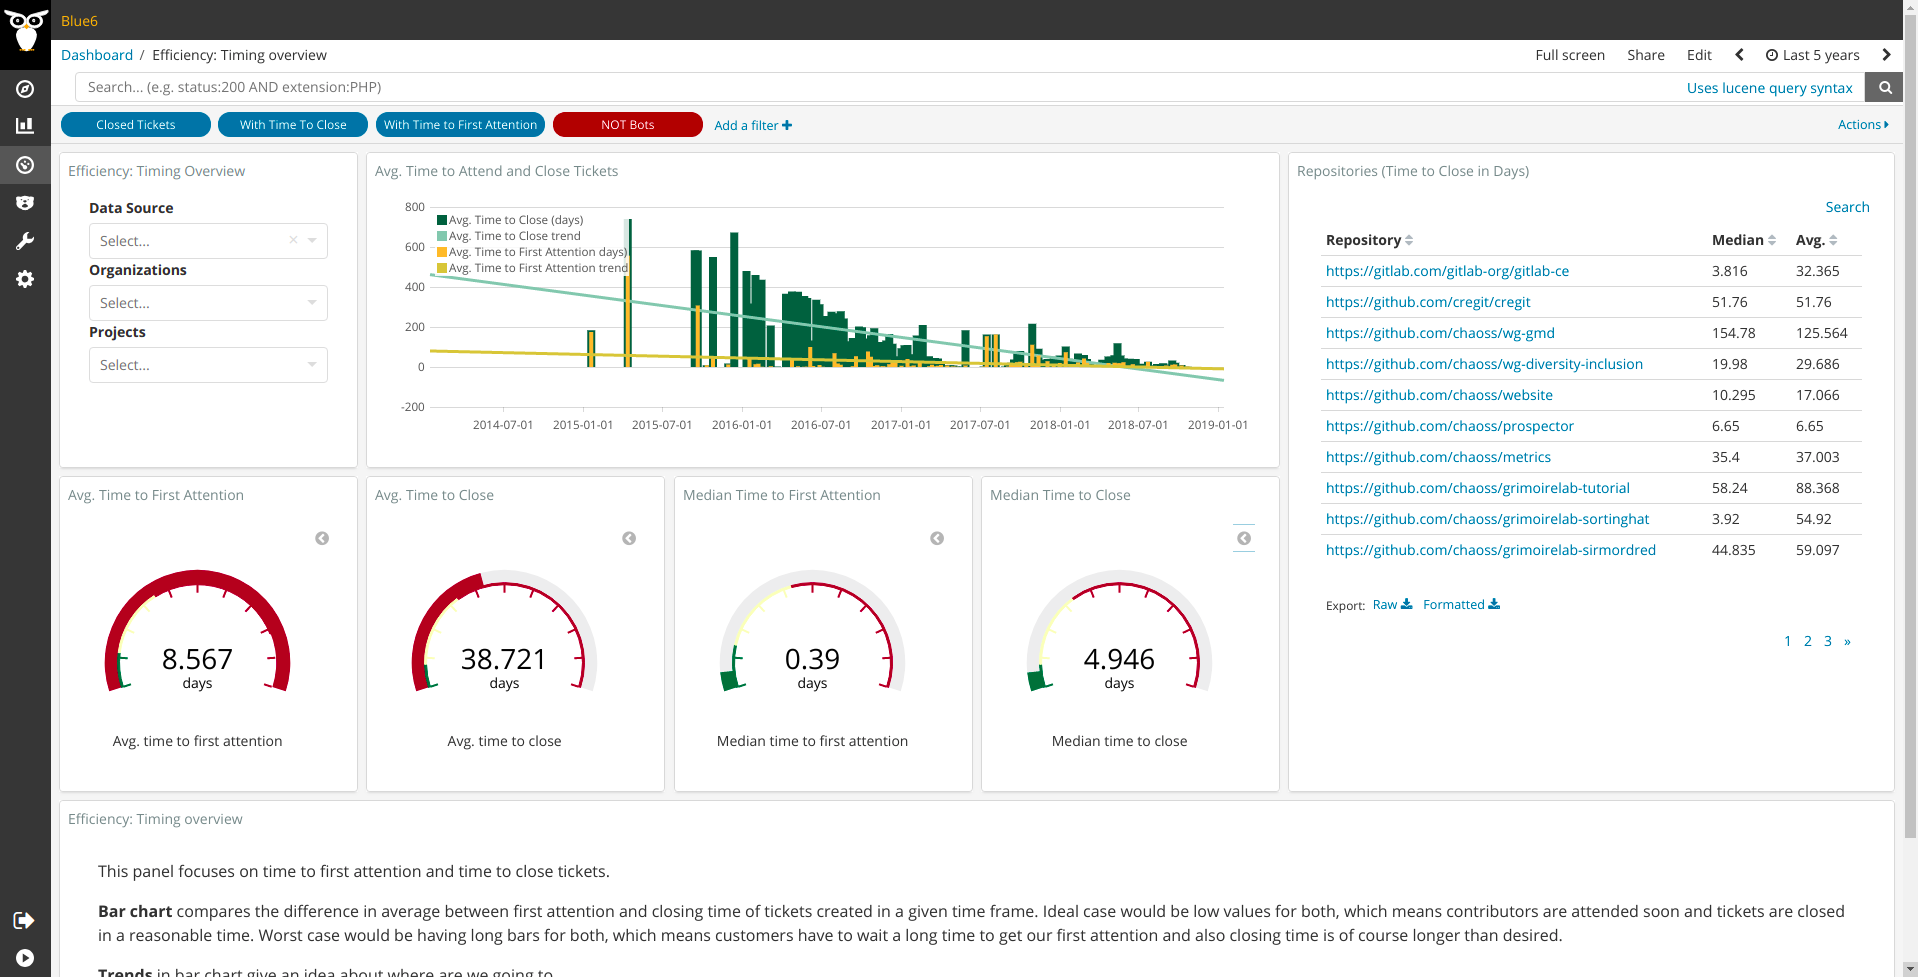
\includegraphics{images/time-to-first-response_efficiency-timing-overview.png}

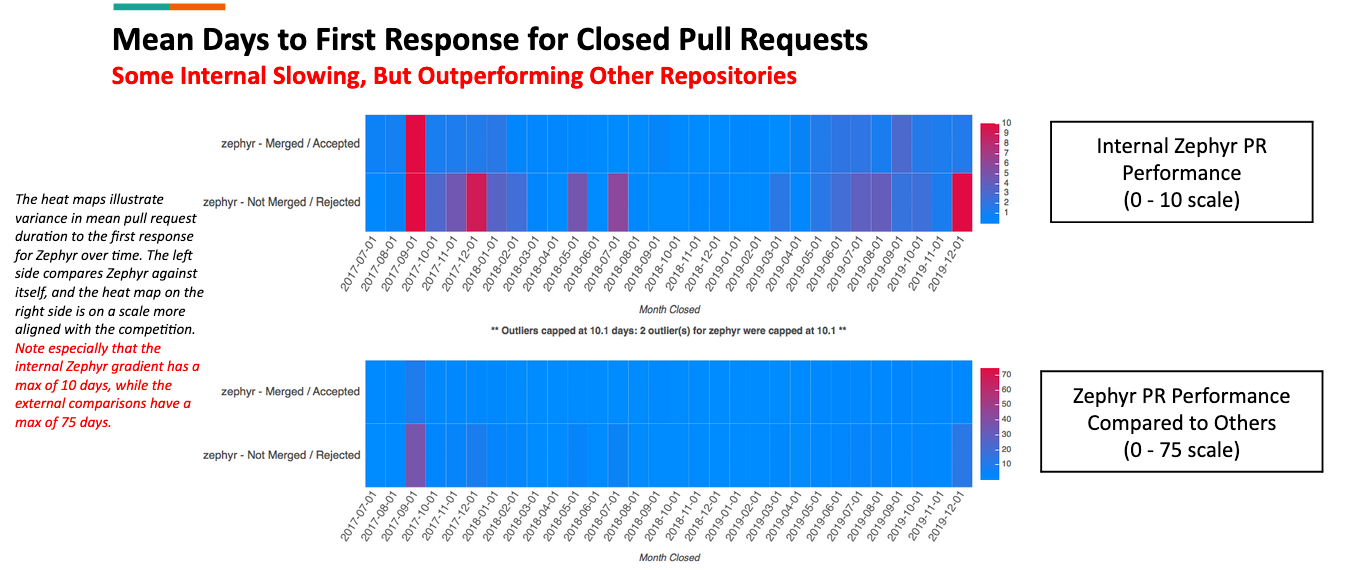
\includegraphics{images/time-to-first-response_augur-ttc-1.png}

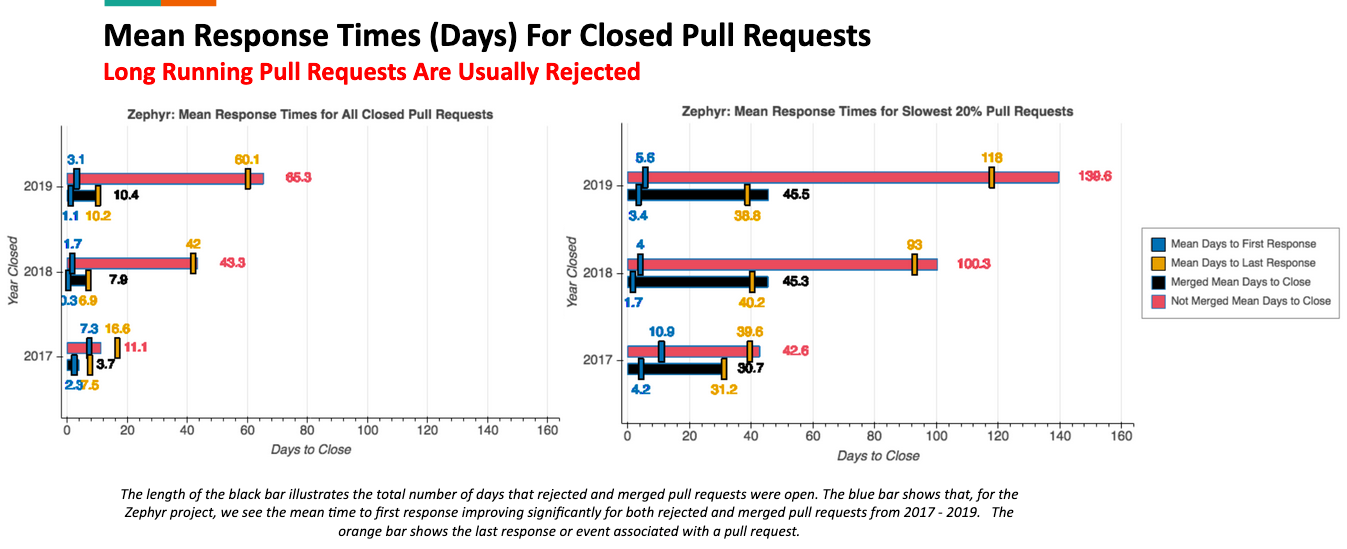
\includegraphics{images/time-to-first-response_augur-ttc-2.png}

\hypertarget{tools-providing-the-metric-4}{%
\subsubsection{Tools Providing the
Metric}\label{tools-providing-the-metric-4}}

\begin{itemize}
\tightlist
\item
  GrimoireLab Panel:
  \href{https://chaoss.github.io/grimoirelab-sigils/panels/efficiency-timing-overview/}{Efficiency
  Timing Overview}
\item
  \href{https://katacontainers.biterg.io/app/kibana\#/dashboard/cbbdd920-288c-11e9-b662-975152e57997}{Kata
  Containers dashboard efficiency panel}
\end{itemize}

\hypertarget{references-6}{%
\subsection{References}\label{references-6}}

\hypertarget{contributor-location}{%
\section{Contributor Location}\label{contributor-location}}

Question: What is the location of contributors?

\hypertarget{description-7}{%
\subsection{Description}\label{description-7}}

Geographical location from which contributors contribute, where they
live, or where they work.

\hypertarget{objectives-7}{%
\subsection{Objectives}\label{objectives-7}}

To determine global locations of contributors in an effort to understand
work practices and times zones. To identify where contributions do not
come from in an effort to improve engagement in these areas.

\hypertarget{implementation-7}{%
\subsection{Implementation}\label{implementation-7}}

\hypertarget{filters-5}{%
\subsubsection{Filters}\label{filters-5}}

Filter contributions by:

\begin{itemize}
\tightlist
\item
  \textbf{Location.} Attempt to group locations in regions to have
  multiple levels of reporting. Location is a purposely ambiguous term
  in this context, and could refer to region, country, state, locale, or
  time zone.
\item
  \textbf{Period of time.} Start and finish date of the period. Default:
  forever. Period during which contributions are counted.
\item
  \textbf{Type of contributor}, for example:

  \begin{itemize}
  \tightlist
  \item
    Repository authors
  \item
    Issue authors
  \item
    Code review participants
  \item
    Mailing list authors
  \item
    Event participants
  \item
    IRC authors
  \item
    Blog authors
  \item
    By release cycle
  \item
    Programming languages of the project
  \item
    Role or function in project
  \end{itemize}
\end{itemize}

\hypertarget{visualizations-6}{%
\subsubsection{Visualizations}\label{visualizations-6}}

Dot Density Map:

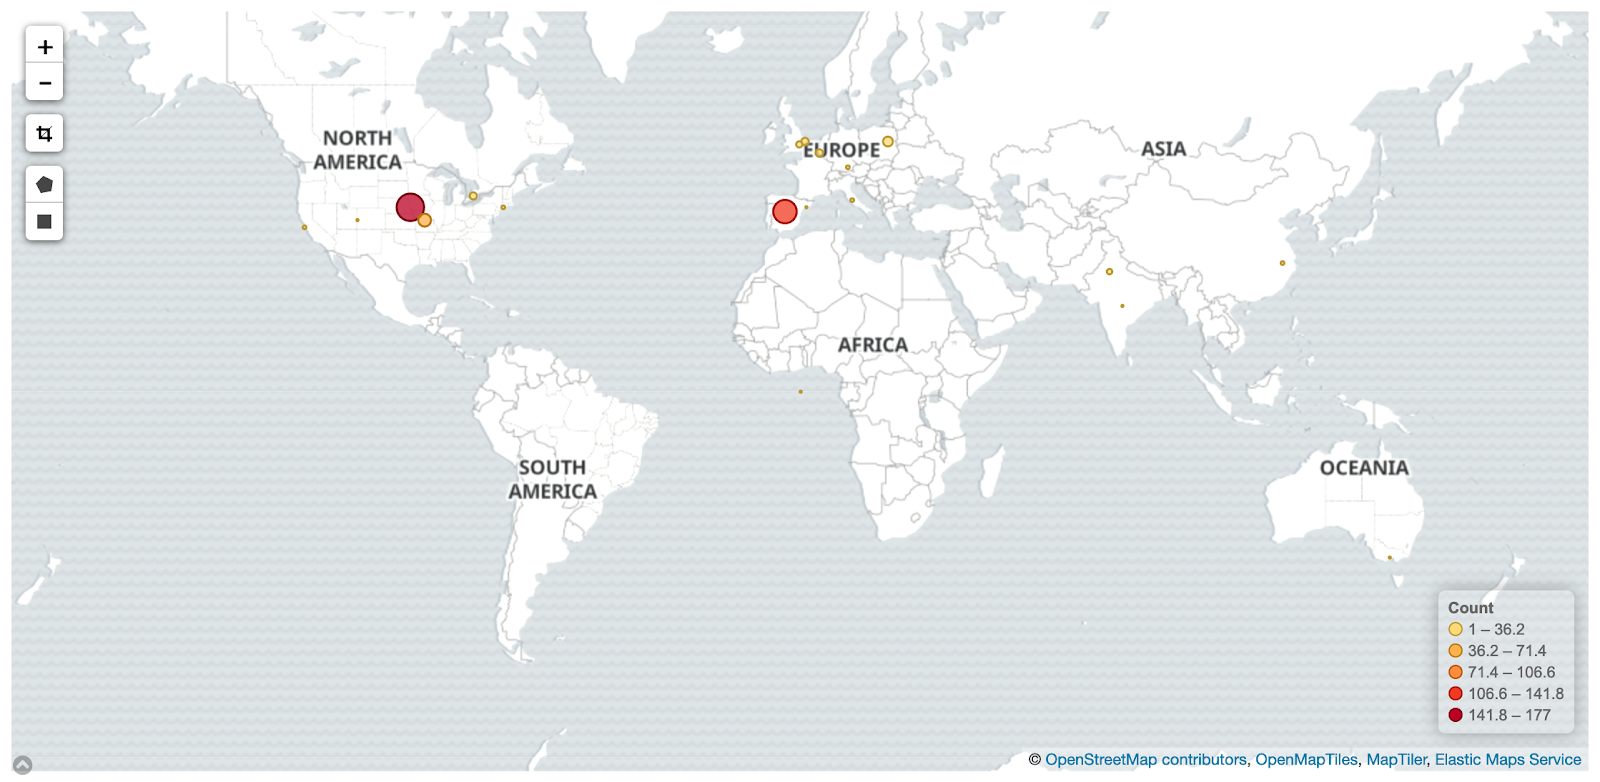
\includegraphics{images/contributor-location_dot-density-map.png}

Source:
\url{https://chaoss.biterg.io/goto/a62f3584a41c1c4c1af5d04b9809a860}

Visual heat map:

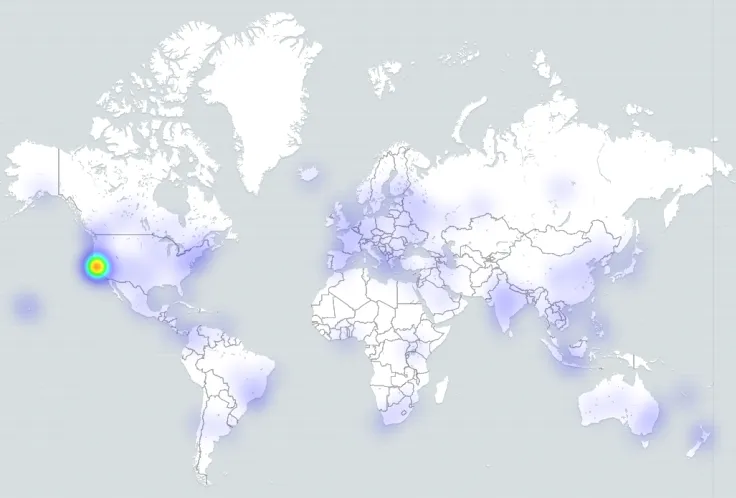
\includegraphics{images/contributor-location_heatmap.png}

Source:
\url{https://blog.bitergia.com/2018/11/20/ubers-community-software-development-analytics-for-open-source-offices}

\hypertarget{tools-providing-the-metric-5}{%
\subsubsection{Tools providing the
metric}\label{tools-providing-the-metric-5}}

\begin{itemize}
\tightlist
\item
  GrimoireLab
\item
  Augur
\end{itemize}

\hypertarget{data-collection-strategies-4}{%
\subsubsection{Data Collection
Strategies}\label{data-collection-strategies-4}}

Different approaches can be used to collect information about location:

\begin{itemize}
\tightlist
\item
  Collect the location information from a contributor's profile in the
  system of engagement.
\item
  Use IP address geolocation of the most frequent locations that
  contributions are made.
\item
  Infer geographical location from the timestamp in contributions.
\item
  Survey contributors.
\end{itemize}

The key challenge for collecting data is determining the location of the
contributor. Best practice would be to leverage any profile information
available from the system of engagement, and if that is not available
then use IP geolocation to determine the most frequent location of
contribution from that individual. Note that contributors may enter in
their profile information false or nonsensical location information
(e.g., ``Earth'' or ``Internet''). Note that IP geolocation can provide
large numbers of false positives due to use of VPNs or other IP masking
tools.

An additional consideration would be the use of external data collection
tools such as community surveys or event registration data that could
cross reference systems of engagement profiles. Contributor location
data could be collected inline with event
\href{https://chaoss.community/metric-attendee-demographics/}{attendee
demographics} and
\href{https://chaoss.community/metric-speaker-demographics/}{speaker
demographics}.

\hypertarget{references-7}{%
\subsection{References}\label{references-7}}

\begin{itemize}
\tightlist
\item
  Gonzalez-Barahona, J. M., Robles, G., Andradas-Izquierdo, R., \&
  Ghosh, R. A. (2008). Geographic origin of libre software developers.
  \emph{Information Economics and Policy}, \emph{20}(4), 356-363.
\end{itemize}

\hypertarget{contributors}{%
\section{Contributors}\label{contributors}}

Question: Who are the contributors to a project?

\hypertarget{description-8}{%
\subsection{Description}\label{description-8}}

A contributor is defined as anyone who contributes to the project in any
way. This metric ensures that all types of contributions are fully
recognized in the project.

\hypertarget{objectives-8}{%
\subsection{Objectives}\label{objectives-8}}

Open source projects are comprised of a number of different
contributors. Recognizing all contributors to a project is important in
knowing who is helping with such activities as code development, event
planning, and marketing efforts.

\hypertarget{implementation-8}{%
\subsection{Implementation}\label{implementation-8}}

Collect author names from collaboration tools a project uses.

\textbf{Aggregators:}

\begin{itemize}
\tightlist
\item
  Count. Total number of contributors during a given time period.
\end{itemize}

\textbf{Parameters:}

\begin{itemize}
\tightlist
\item
  Period of time. Start and finish date of the period. Default: forever.
  Period during which contributions are counted.
\end{itemize}

\hypertarget{filters-6}{%
\subsubsection{Filters}\label{filters-6}}

By location of engagement. For example:

\begin{itemize}
\tightlist
\item
  Commit authors
\item
  Issue authors
\item
  Review participants, e.g., in pull requests
\item
  Mailing list authors
\item
  Event participants
\item
  IRC authors
\item
  Blog authors
\item
  By release cycle
\item
  Timeframe of activity in the project, e.g, find new contributors
\item
  Programming languages of the project
\item
  Role or function in project
\end{itemize}

\hypertarget{visualizations-7}{%
\subsubsection{Visualizations}\label{visualizations-7}}

\begin{itemize}
\tightlist
\item
  List of contributor names (often with information about their level of
  engagement)
\end{itemize}

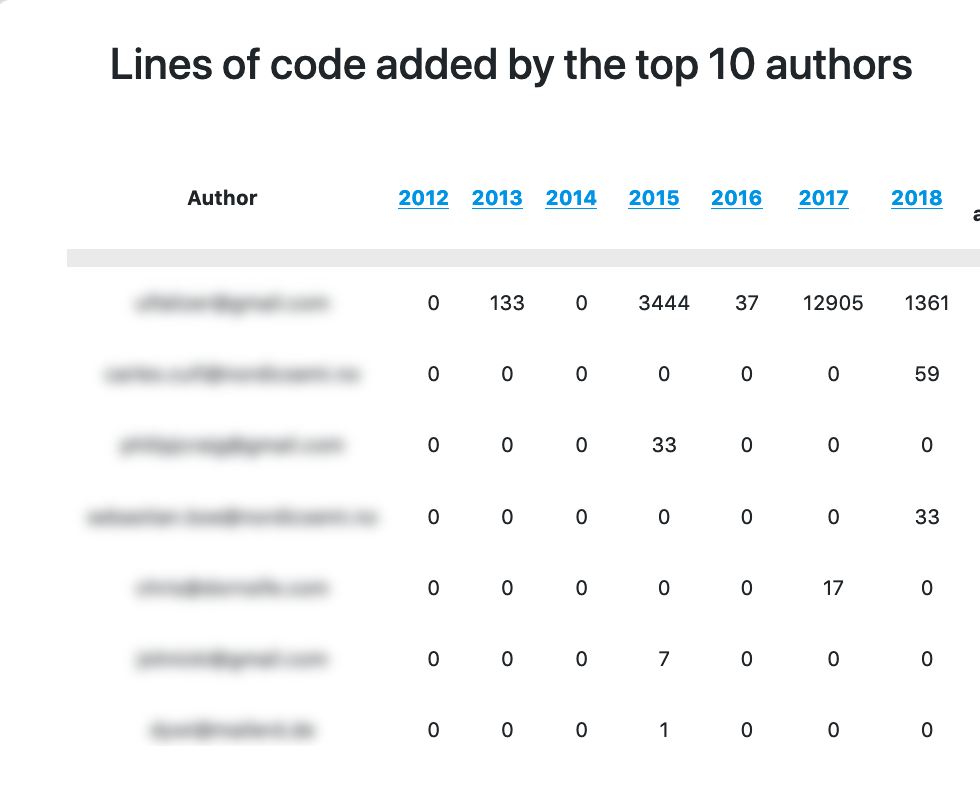
\includegraphics{images/contributors_top-contributor-info.png}

\begin{itemize}
\tightlist
\item
  Summary number of contributors
\end{itemize}

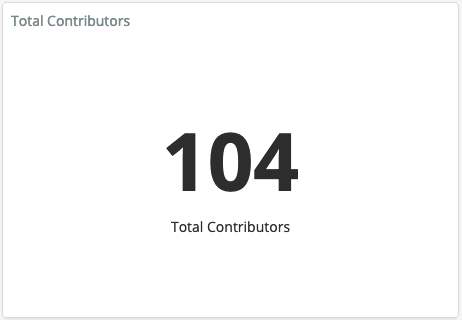
\includegraphics{images/contributors_summary-contributor-number.png}

\begin{itemize}
\tightlist
\item
  Change in the number of active contributors over time
\end{itemize}

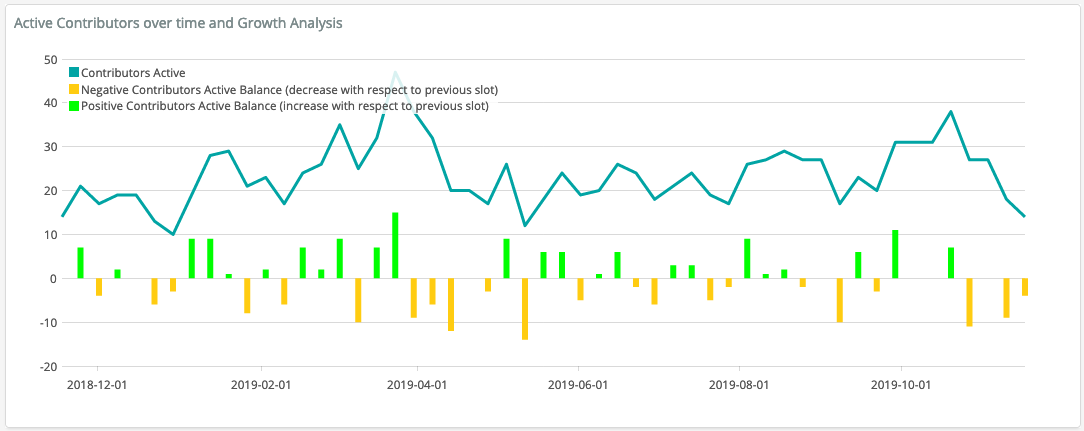
\includegraphics{images/contributors_growth.png}

\begin{itemize}
\tightlist
\item
  New contributors (sort list of contributors by date of first
  contribution)
\end{itemize}

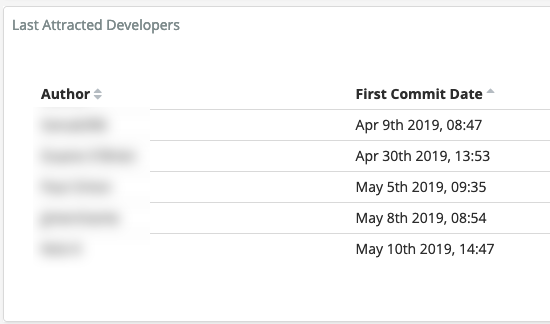
\includegraphics{images/contributors_first-commit-date.png}

\hypertarget{tools-providing-the-metric-6}{%
\subsubsection{Tools Providing the
Metric}\label{tools-providing-the-metric-6}}

\begin{itemize}
\tightlist
\item
  \href{https://chaoss.github.io/grimoirelab/}{GrimoireLab}
\item
  \href{http://augur.osshealth.io/api_docs/\#api-Evolution-Contributors_Repo_}{Augur}
\end{itemize}

\hypertarget{data-collection-strategies-5}{%
\subsubsection{Data Collection
Strategies}\label{data-collection-strategies-5}}

As indicated above, some contributor information is available via
software such as GrimoireLab and Augur. However, some contributor
insights are less easily obtained via trace data. In these cases,
surveys with community members or event registrations can provide the
desired information. Sample questions include:

\begin{itemize}
\tightlist
\item
  Interview question: Which contributors do not typically appear in
  lists of contributors?
\item
  Interview question: Which contributors are often overlooked as
  important contributors because their contributions are more ``behind
  the scenes''?
\item
  Interview question: What other community members do you regularly work
  with?
\end{itemize}

Additionally, surveys with community members can provide insight to
learn more about contributions to the project. Sample questions include:

\begin{itemize}
\tightlist
\item
  Likert scale {[}1-x{]} item: I am contributing to the project
\item
  Matrix survey item: How often do you engage in the following
  activities in the project?

  \begin{itemize}
  \tightlist
  \item
    Column headings: Never, Rarely(less than once a month), Sometimes
    (more than once a month), Often(once a week or more)
  \item
    Rows include: a) Contributing/reviewing code, b) Creating or
    maintaining documentation, c) Translating documentation, d)
    Participating in decision making about the project's development, e)
    Serving as a community organizer, f) Mentoring other contributors,
    g) Attending events in person, h) Participating through school or
    university computing programs, i) Participating through a program
    like Outreachy, Google Summer of Code, etc., j) Helping with the ASF
    operations (e.g., board meetings or fundraising)
  \end{itemize}
\end{itemize}

\hypertarget{references-8}{%
\subsection{References}\label{references-8}}

\hypertarget{organizational-diversity}{%
\section{Organizational Diversity}\label{organizational-diversity}}

Question: What is the organizational diversity of contributions?

\hypertarget{description-9}{%
\subsection{Description}\label{description-9}}

Organizational diversity expresses how many different organizations are
involved in a project and how involved different organizations are
compared to one another.

\hypertarget{objectives-9}{%
\subsection{Objectives}\label{objectives-9}}

\begin{itemize}
\tightlist
\item
  Get a list of organizations contributing to a project.
\item
  See the percentage of contributions from each organization within a
  defined period of time.
\item
  See the change of composition of organizations within a defined period
  of time.
\item
  Get a list of people that are associated with each organization.
\end{itemize}

\hypertarget{implementation-9}{%
\subsection{Implementation}\label{implementation-9}}

\begin{itemize}
\tightlist
\item
  Collect data from data sources where contributions occur.
\item
  Identify contributor affiliations to get a good estimate of which
  organizations they belong to.
\item
  Correlate information about contributions, assigning each to
  appropriate organization.
\item
  Depending on the needs of the project, you may want to consider such
  issues as how to handle multiple email addresses, affiliation changes
  over time, or contractor vs. employee.
\end{itemize}

\hypertarget{tools-providing-the-metric-7}{%
\subsubsection{Tools Providing the
Metric}\label{tools-providing-the-metric-7}}

\begin{itemize}
\tightlist
\item
  \href{https://chaoss.github.io/grimoirelab}{GrimoireLab} supports
  organizational diversity metrics out of the box. The
  \href{https://github.com/chaoss/grimoirelab-sortinghat}{GrimoireLab
  SortingHat} manages identities. The
  \href{https://github.com/chaoss/grimoirelab-hatstall}{GrimoireLab
  Hatstall} user interface allows correcting organizational affiliation
  of people and even recording affiliation changes.

  \begin{itemize}
  \tightlist
  \item
    View an example visualization on the
    \href{https://chaoss.biterg.io/app/kibana\#/dashboard/Community-Structure-by-Organization}{CHAOSS
    instance of Bitergia Analytics}.
  \item
    Download and import a ready-to-go dashboard containing examples for
    this metric visualization from the
    \href{https://chaoss.github.io/grimoirelab-sigils/panels/community-structure-by-organization/}{GrimoireLab
    Sigils panel collection}.
  \item
    Add a sample visualization to any GrimoreLab Kibiter dashboard
    following these instructions:

    \begin{itemize}
    \tightlist
    \item
      Create a new Pie chart

      \begin{itemize}
      \tightlist
      \item
        Select the \texttt{all\_onion} index
      \item
        Metrics Slice Size: \texttt{Sum} Aggregation,
        \texttt{contributions} Field, \texttt{Contributions} Custom
        Label
      \item
        Buckets Split Slices: \texttt{Terms} Aggregation,
        \texttt{author\_or\_name} Field, \texttt{metric:\ Contributions}
        Order By, \texttt{Descending} Order, \texttt{500} Size,
        \texttt{Organization} Custom Label
      \end{itemize}
    \item
      Example Screenshot
    \end{itemize}

    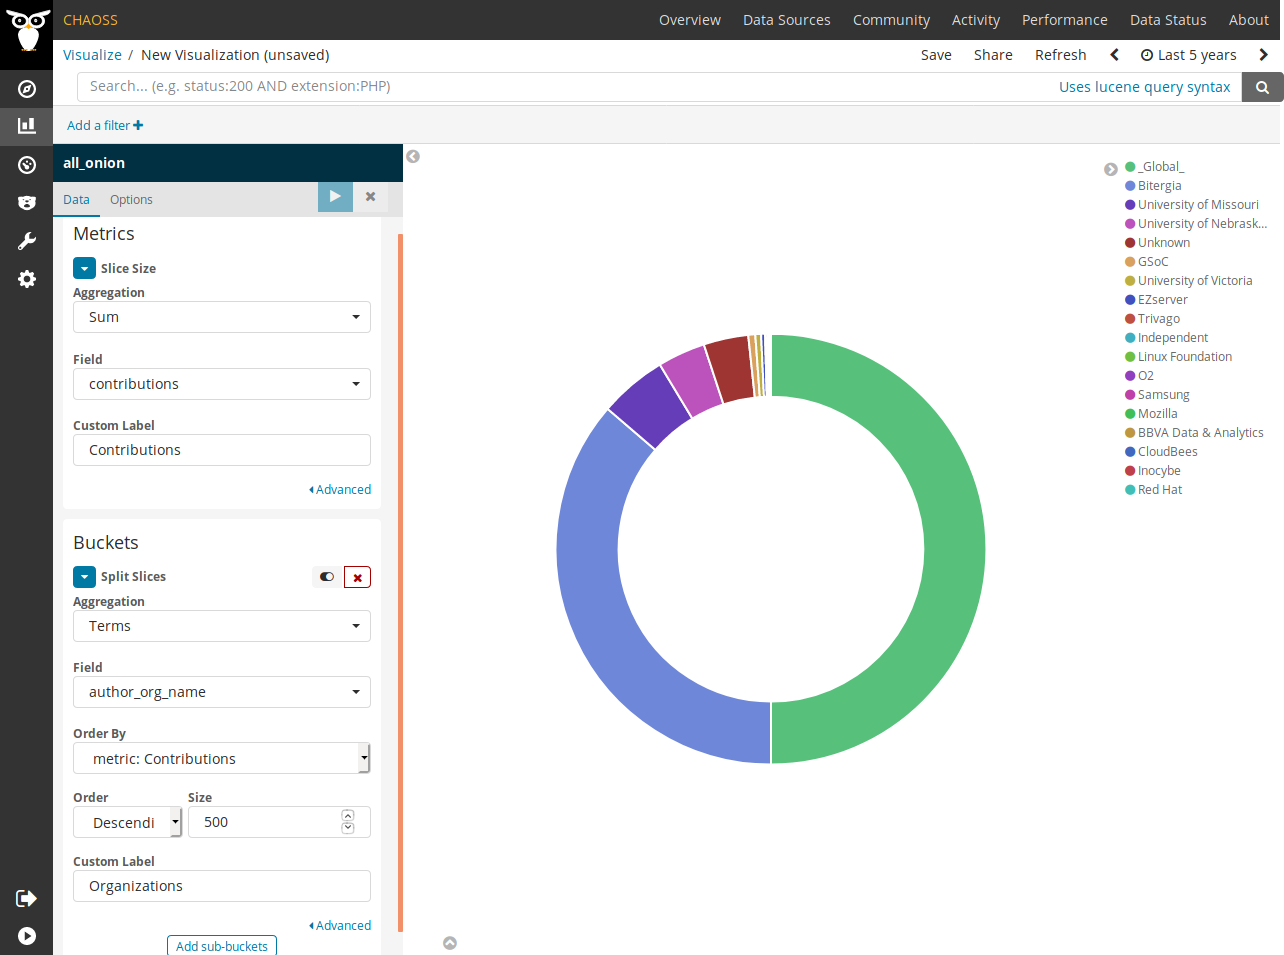
\includegraphics{images/organizational-diversity_piechart.png}
  \end{itemize}
\item
  \href{https://lfanalytics.io}{LF Analytics} provides organization
  diversity metrics in the primary view for commits, issues filed, and
  communication channels (current support for Slack and groups.io)
\end{itemize}

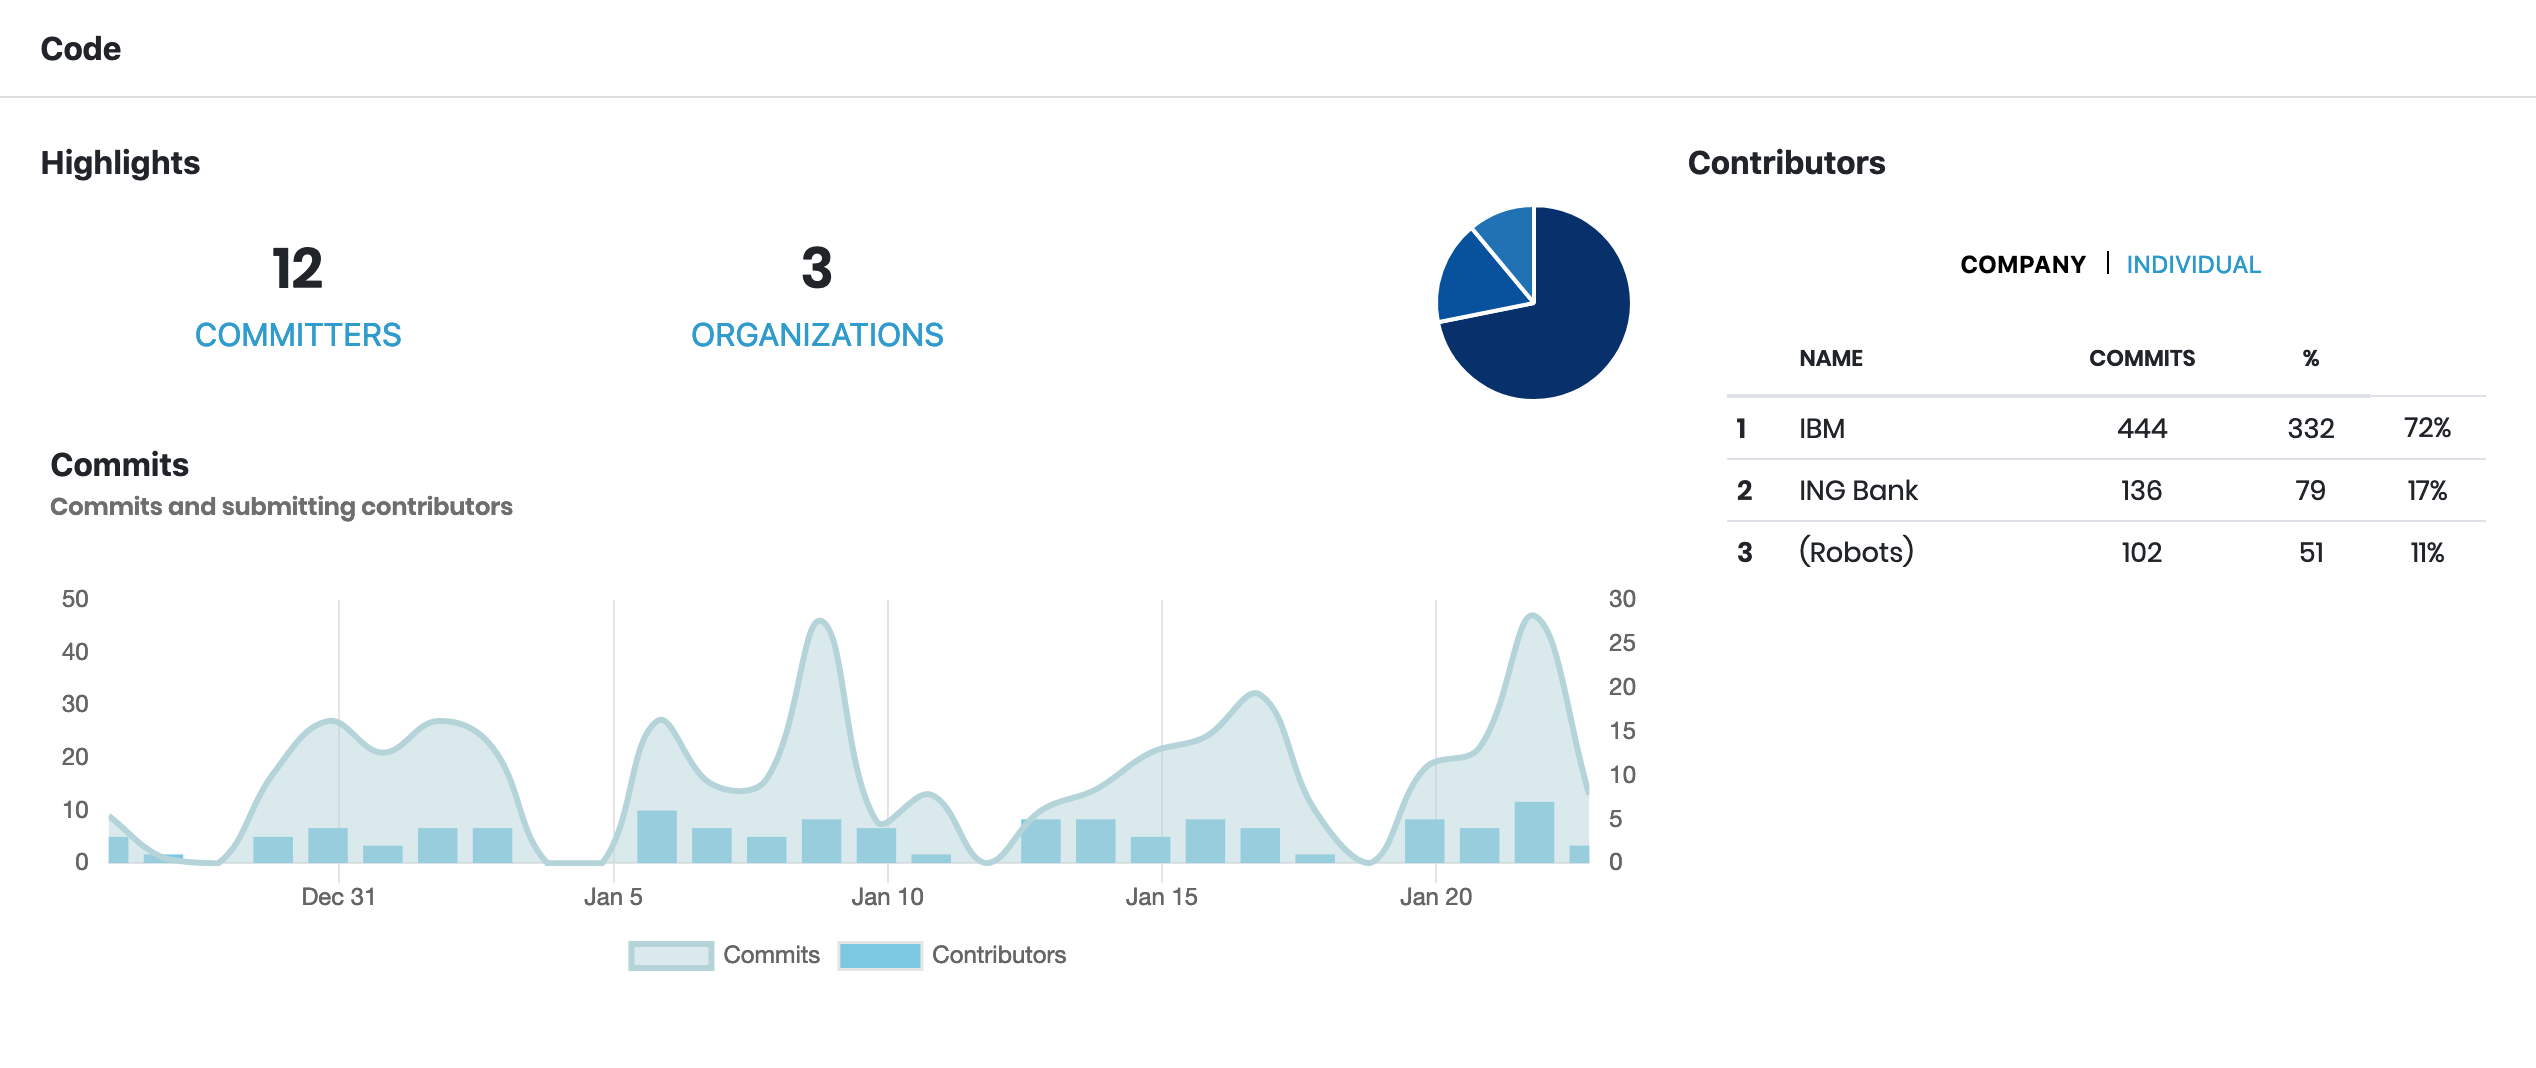
\includegraphics{images/organizational-diversity_lfanalytics-orgdiversity.png}

\hypertarget{data-collection-strategies-6}{%
\subsubsection{Data Collection
Strategies}\label{data-collection-strategies-6}}

\textbf{Qualitative}

\begin{itemize}
\tightlist
\item
  Footprint of an organization in a project or ecosystem
\item
  Influence of an organization in a project or ecosystem
\item
  Affiliation diversity in governance structures.
\end{itemize}

\textbf{Quantitative}

\begin{itemize}
\tightlist
\item
  \% of commits by each organization
\item
  \% of merges/reviews from each organization
\item
  \% of any kind of contributors from each organization
\item
  \% of lines of code contributed by each organization
\item
  \% issues filed by each organization
\item
  \href{https://github.com/chaoss/metrics/blob/master/activity-metrics/contributing-organizations.md}{Contributing
  Organizations} - What is the number of contributing organizations?
\item
  \href{https://github.com/chaoss/metrics/blob/master/activity-metrics/new-contributing-organizations.md}{New
  Contributing Organizations} - What is the number of new contributing
  organizations?
\item
  New Contributor Organizations - New organizations contributing to the
  project over time.
\item
  Number of Contributing Organizations - Number of organizations
  participating in the project over time.
\item
  Elephant Factor - If 50\% of community members are employed by the
  same company, it is the elephant in the room. Formally: The minimum
  number of companies whose employees perform 50\% of the commits
\item
  \href{https://github.com/chaoss/metrics/blob/master/activity-metrics/contributor-diversity.md}{Affiliation
  Diversity} - Ratio of contributors from a single company over all
  contributors. Also described as: Maintainers from different companies.
  Diversity of contributor affiliation.
\item
  In projects with the concept of code ownership, \% of code owners
  affiliated with each organization weighed by the importance/size/LoC
  of the code they own and the number of co-owners.
\end{itemize}

\hypertarget{references-9}{%
\subsection{References}\label{references-9}}

\begin{itemize}
\tightlist
\item
  Potential implementations and references:

  \begin{itemize}
  \tightlist
  \item
    \url{https://bitergia.gitlab.io/panel-collections/open_source_program_office/organizational-diversity.html}
  \item
    \href{https://katacontainers.biterg.io}{Kata Containers dashboard
    entry page} (bottom of this)
  \item
    \href{https://github.com/chaoss/augur}{Augur}
  \end{itemize}
\end{itemize}

\end{document}
